\titledquestion{Distance Measurement on a Graph}
Given a weighted Digraph $D = (V,A,c_{ij})$:
\begin{figure}[ht]%
\centering
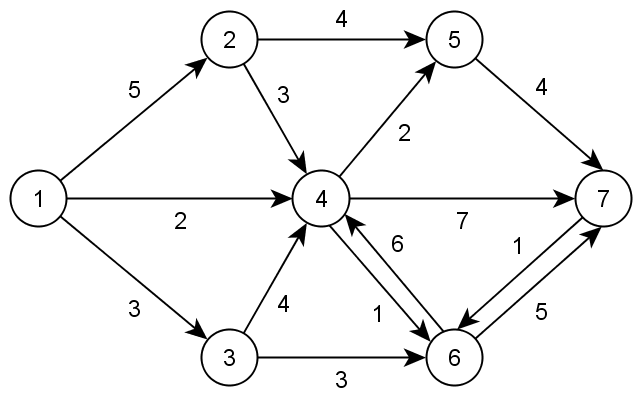
\includegraphics[scale=.2]{Uebungen/figures/digraph}%
\end{figure}

\begin{enumerate}
	\item Using Dijkstra's algorithm, determine shortest paths and distances $d(s,i)$ starting from the source $s = 1$ to all other nodes $i=2,\ldots,7$ !
	
	\begin{solution}
	Initialization $d_i=\infty$ for all nodes i.
	\begin{center}
			\begin{tabular}{c|c|c|c}
			Iteration&Selected Node i&Temporarily marked Nodes&New Label\\
			\hline
			0&-&$s=1$&$d\left(1\right)=0$\\
			1&\phantom{1}&\phantom{$2,3,4$}&\phantom{$d\left(2\right)=5$, $d\left(3\right)=3$, $d\left(4\right)=2$}\\
			2&\phantom{4}&\phantom{$2,3,5,6,7$}&\phantom{$d\left(5\right)=4$, $d\left(6\right)=3$, $d\left(7\right)=9$}\\
			3&\phantom{3}&\phantom{$2,5,6,7$}&\\
			4&\phantom{6}&\phantom{$2,5,7$}&\phantom{$d\left(7\right)=8$}\\
			5&\phantom{5}&\phantom{$2,7$}&\\
			6&\phantom{2}&\phantom{$7$}&\\
			7&\phantom{7}&\phantom{-}&\\
			\end{tabular}
		\end{center}
	\uline{Output:}
	\begin{center}
		\begin{tabular}{|c|ccccccc|}
		\hline
		Node i&1&2&3&4&5&6&7\\
		\hline
		pred(i)&\phantom{-}&\phantom{1}&\phantom{1}&\phantom{1}&\phantom{4}&\phantom{4}&\phantom{6}\\
		\hline
		d(i)&\phantom{0}&\phantom{5}&\phantom{3}&\phantom{2}&\phantom{4}&\phantom{3}&\phantom{8}\\
		\hline
		\end{tabular}
	\end{center}
	\end{solution}
	
	\item What happens if the condition $c_{ij} \geq 0$ is not satisfied? Construct a (small) example.
	\begin{solution}
	
	Example:
	\begin{center}
		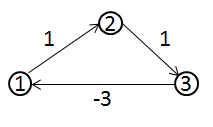
\includegraphics[scale=0.7]{Uebungen/figures/Graph_A_3_2}
	\end{center}
	Initialization $d_i=\infty$ for all nodes i
	\begin{center}
			\begin{tabular}{c|c|c|c}
			Iteration&Selected Node i&Temporarily Marked Nodes&New Label\\
			\hline
			0&-&$s=1$&$d\left(1\right)=0$\\
			1&\phantom{1}&\phantom{$2$}&\phantom{$d\left(2\right)=1$}\\
			2&\phantom{2}&\phantom{$3$}&\phantom{$d\left(3\right)=2$}\\
			3&\phantom{3}&\phantom{-}&\phantom{$d\left(1\right)=-1$}\\
			\end{tabular}
		\end{center}
		\textbf{Observation:}
	\begin{itemize}
	\item Node 1 is already visited. Nevertheless, one can still find a shorter (arbitrarily many) path(s) to this node.
	\item This is due to the fact that $c_{31}-d(3)<0$.
\end{itemize}
	
	\textbf{Note:}  If $c_{ij}\geq 0$ holds for all nodes $i,j$, then
	\begin{itemize}
			\item every node reachable from s is included exactly once in $L$ (set of temporarily marked nodes).
			\item the $d(i)$ of visited node $i$, already eliminated from $L$, cannot be further reduced.
	\end{itemize}
	\end{solution}
\end{enumerate}
\begin{enumerate}
\setcounter{enumi}{2}
	\item Is Dijkstra's algorithm also applicable to weighted undirected graphs, e.g., to the following graph $G = (V,E,c_{ij})$? What modifications, if any, would need to be made?
\begin{figure}[h]%
\centering
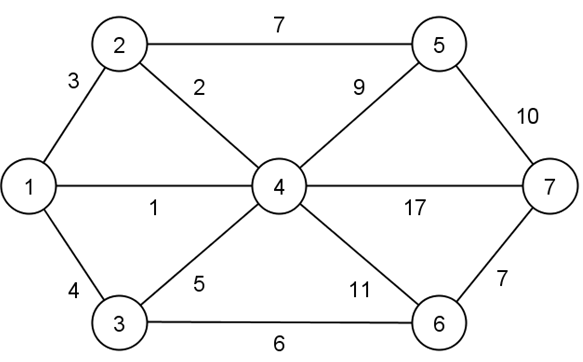
\includegraphics[scale=.4]{Uebungen/figures/Graph}
\end{figure}
	\begin{solution}
	In principle, Dijkstra's algorithm is also applicable to weighted undirected graphs if you replace each edge by two anti-parallel arcs and weight them with $c_{ij}=c_{ji}$.
	\end{solution}

Now a facility $q$ is to be placed somewhere on the edge $e=\{1,4\}$. For a reminder, the extended distance function for a point $q=q(\{i,j\},\lambda)$ where $q$ lies somewhere along the edge $\{i,j\}\in E$ is given by:
	\[
	d\left(q,k\right) := \min\{\lambda c_{ij} + d\left(i,k\right), (1 - \lambda) c_{ij} + d(j,k) \} \, ,
	\]
with (real) Parameter $0 \leq \lambda \leq 1$ used to define where $q$ lies along the edge $\{i,j\}\in E$.
	\item Determine the distance $d(q,7)$ for $\lambda_1=0,\lambda_2=0.5$ and $\lambda_3=1$! What do you observe? Does this observation for $\lambda = 0.5$ also apply in general?
	\begin{solution}
	\uline{Procedure:}
		\begin{enumerate}
			\item Calculate the edge segments:
				\begin{itemize}
					\item $d\left(q,i\right)=\lambda c_{ij}$
					\item $d\left(q,j\right)=\left(1-\lambda\right)c_{ij}$
				\end{itemize}
			\item Calculate the shortest distances for $d\left(i,k\right)$ and $d\left(j,k\right)$ using e.g. Dijkstra's algorithm.
			\item Add the corresponding edge segment and shortest distance:
				\begin{itemize}
					\item $q\rightarrow i\rightarrow k$: $d\left(q,i\right)+d\left(i,k\right)$
					\item $q\rightarrow j\rightarrow k$: $d\left(q,j\right)+d\left(j,k\right)$
				\end{itemize}
			\item Choose the path with the shortest distance.
		\end{enumerate}
		\uline{Calculation:}\\
		\begin{center}
			\begin{tabular}{c|c|c|c}
			&$\lambda_1=0$&$\lambda_2=0,5$&$\lambda_3=1$\\
			\hline
			$d\left(q,i\right)$&0&0,5&1\\
			$d\left(q,j\right)$&1&0,5&0\\
			$d\left(i,k\right)$&17&17&17\\
			$d\left(j,k\right)$&17&17&17\\
			$d\left(q,i\right)+d\left(i,k\right)$&17&17,5&18\\
			$d\left(q,j\right)+d\left(j,k\right)$&18&17,5&17\\
			\end{tabular}
		\end{center}
	\uline{Observation:}\\
	
	The path from facility $q$ to node $7$ is of equal length via nodes $1$ and $4$ for $\lambda_2=0,5$.\\
	
	No, the observation for $\lambda_2=0.5$ does not hold in general. It is only valid in this example, because $d\left(i,k\right)=d\left(j,k\right)$. E.g., for the edge $f=\{3,4\}$ it follows with $d(3,7)= 13 \neq 17 = d(4,7)$:
		\begin{center}
		\begin{tabular}{c|c|c|c}
			&$\lambda_1=0$&$\lambda_2=0,5$&$\lambda_3=1$\\
			\hline
			$d\left(q,i\right)$&0&2,5&5\\
			$d\left(q,j\right)$&5&2,5&0\\
			$d\left(i,k\right)$&13&13&13\\
			$d\left(j,k\right)$&17&17&17\\
			$d\left(q,i\right)+d\left(i,k\right)$&13&15,5&18\\
			$d\left(q,j\right)+d\left(j,k\right)$&22&19,5&17\\
		\end{tabular}
	\end{center}
	\end{solution}
\end{enumerate}